% Indicate the main file. Must go at the beginning of the file.
% !TEX root = ../main.tex

%%%%%%%%%%%%%%%%%%%%%%%%%%%%%%%%%%%%%%%%%%%%%%%%%%%%%%%%%%%%%%%%%%%%%%%%%%%%%%%%
% 06_acknowledgment_declaration
%%%%%%%%%%%%%%%%%%%%%%%%%%%%%%%%%%%%%%%%%%%%%%%%%%%%%%%%%%%%%%%%%%%%%%%%%%%%%%%%


\section{Acknowledgment and Declaration}
\label{acknowledgment_declaration}

\subsection{Acknowledgment}%%%%%%%%%%%%%%%%%%%%%%%%%%%%%%%%%%%%%%%%%%%%%%%%%%%%%%

I am deeply grateful to my supervisor, Dr. Stefan Glüge, for his invaluable guidance and interesting discussions throughout this thesis. 
My thanks also go to Dr. Matthias Nyfeler, who provided the topic and ensured I had all the support needed troughout the project. 
I want to thank Prof. Dr. Roland Felix Graf and Nils Ratnaweera for their help in obtaining the data and all the information I needed on the Wildlife@Campus project to get started with the thesis. 
Finally, I would like to thank the HPC-support team --- especially Dr. Pascal Häussler --- for their assistance with the cluster and their impressively swift responses to my questions.

\subsection{Declaration of AI Usage}%%%%%%%%%%%%%%%%%%%%%%%%%%%%%%%%%%%%%%%%%%%%%%

\textbf{GitHub Copilot} was active for all the coding tasks as well as for the text writing in this thesis.
While for the texting it was mainly intended to assist with the LaTeX formatting, it also provided suggestions for the text itself.
For the actual coding task it was used to assist solving problems, writing code snippets and played a significant role debugging the code.
\textbf{ChatGPT Model o4-mini} was used to assist writing code, solving problems and debugging issues.
\textbf{ChatGPT GPT-4o} and \textbf{GPT-4.5} where used to assist researching content, structuring the thesis, writing and streamlining the text.
Every paragraph was finally feed into the \textbf{GPT-4o} for a final spelling and grammar check --- the changes where all reviewed manually utilizing the git diff viewer to ensure no unwanted changes where introduced.

\newpage
\refstepcounter{subsection}
\addcontentsline{toc}{subsection}{\protect\numberline{\thesubsection}Statement of Authorship}

\newgeometry{left=0in, right=0in, top=0.5in, bottom=0in}
\thispagestyle{empty}
\begin{figure}[h!]
    \centering
    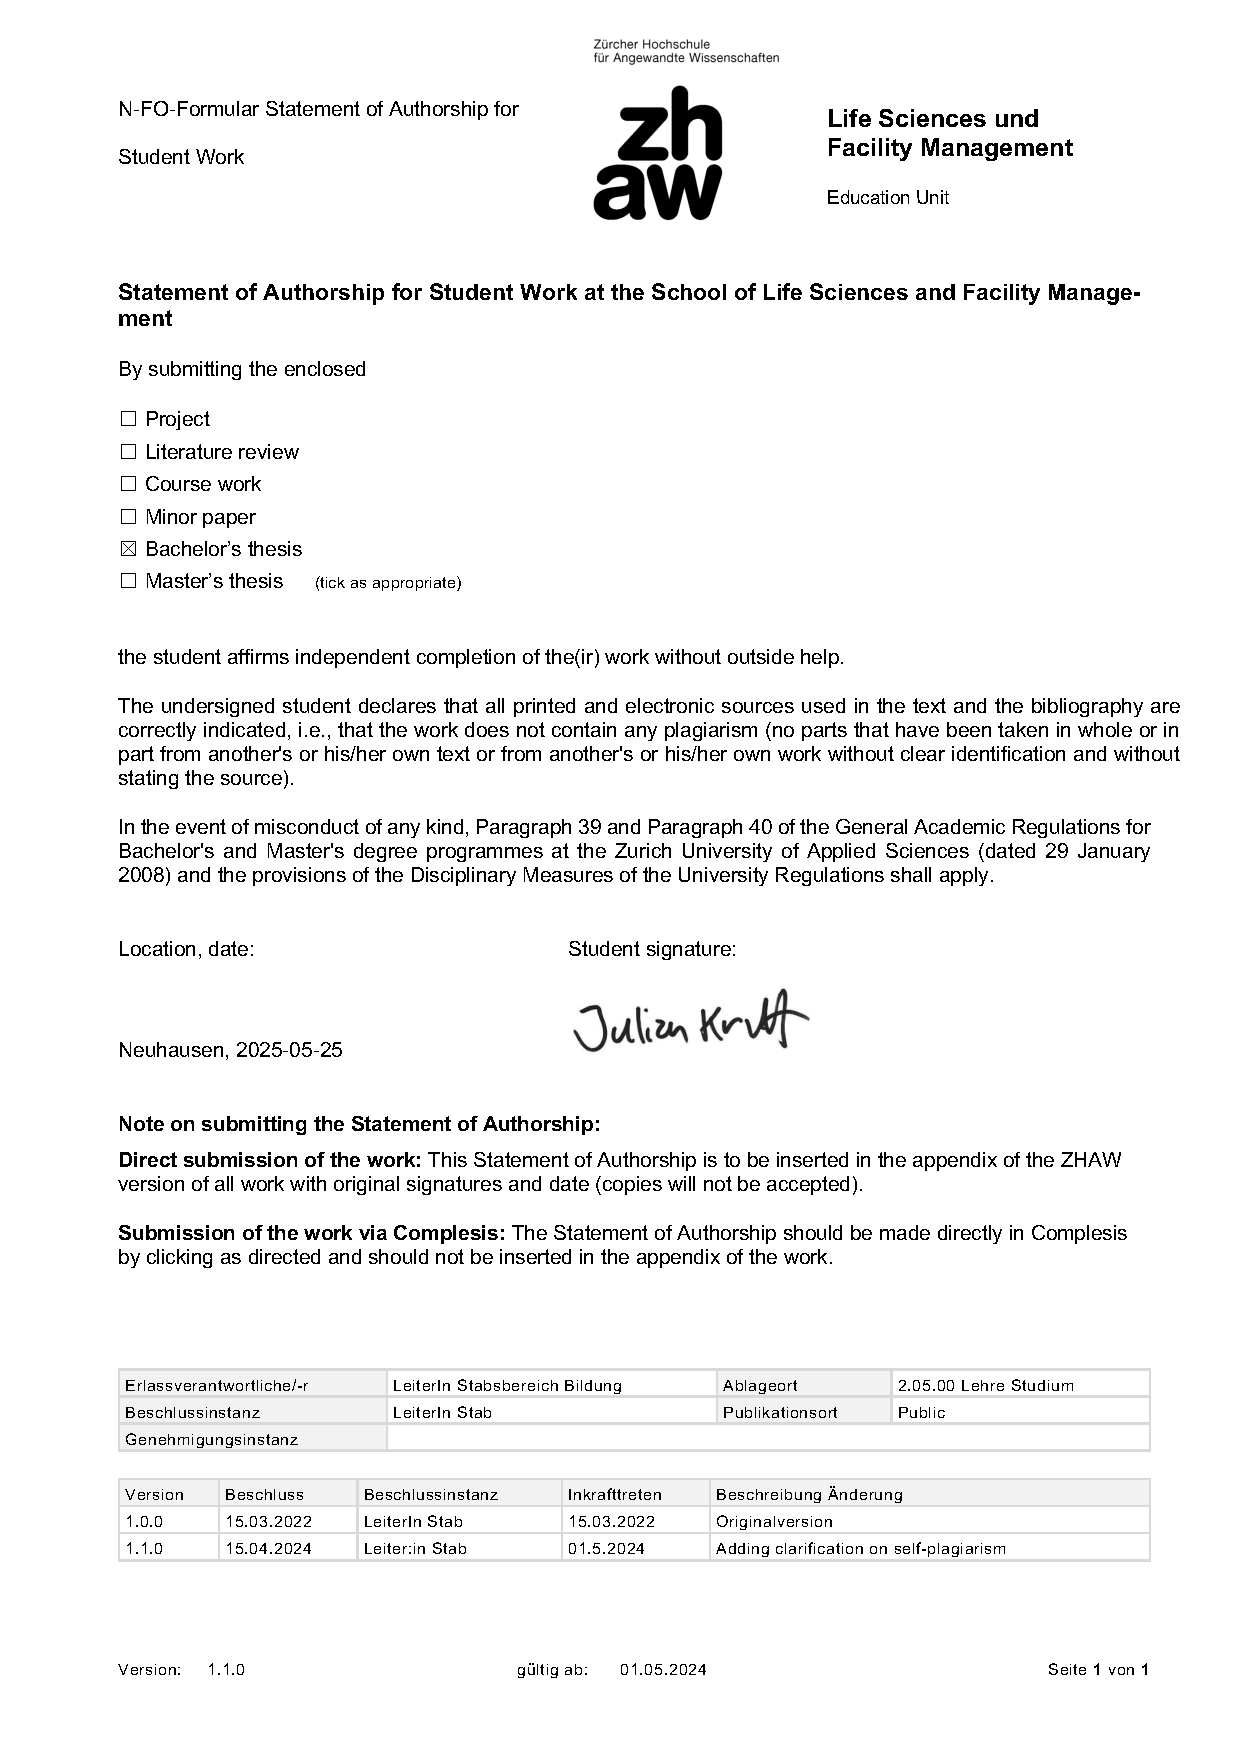
\includegraphics[width=0.9\textwidth]{figures/declaration_independence.pdf}
\end{figure}
\restoregeometry % Restore original margins
